% Generated by benchmarks/src/utils/make_table4_speedup_figures.py -- do not hand-edit.
\definecolor{sp0}{HTML}{2A78D6}
\definecolor{sp1}{HTML}{EB6834}
\definecolor{sp2}{HTML}{1BAF7A}
\pgfdeclareplotmark{heptagon*}{\pgfpathmoveto{\pgfqpointpolar{90.00}{\pgfplotmarksize}}\pgfpathlineto{\pgfqpointpolar{141.43}{\pgfplotmarksize}}\pgfpathlineto{\pgfqpointpolar{192.86}{\pgfplotmarksize}}\pgfpathlineto{\pgfqpointpolar{244.29}{\pgfplotmarksize}}\pgfpathlineto{\pgfqpointpolar{295.71}{\pgfplotmarksize}}\pgfpathlineto{\pgfqpointpolar{347.14}{\pgfplotmarksize}}\pgfpathlineto{\pgfqpointpolar{38.57}{\pgfplotmarksize}}\pgfpathclose\pgfusepathqfill}
\pgfdeclareplotmark{octagon*}{\pgfpathmoveto{\pgfqpointpolar{90.00}{\pgfplotmarksize}}\pgfpathlineto{\pgfqpointpolar{135.00}{\pgfplotmarksize}}\pgfpathlineto{\pgfqpointpolar{180.00}{\pgfplotmarksize}}\pgfpathlineto{\pgfqpointpolar{225.00}{\pgfplotmarksize}}\pgfpathlineto{\pgfqpointpolar{270.00}{\pgfplotmarksize}}\pgfpathlineto{\pgfqpointpolar{315.00}{\pgfplotmarksize}}\pgfpathlineto{\pgfqpointpolar{0.00}{\pgfplotmarksize}}\pgfpathlineto{\pgfqpointpolar{45.00}{\pgfplotmarksize}}\pgfpathclose\pgfusepathqfill}
\begin{figure*}[!t]
    \centering
    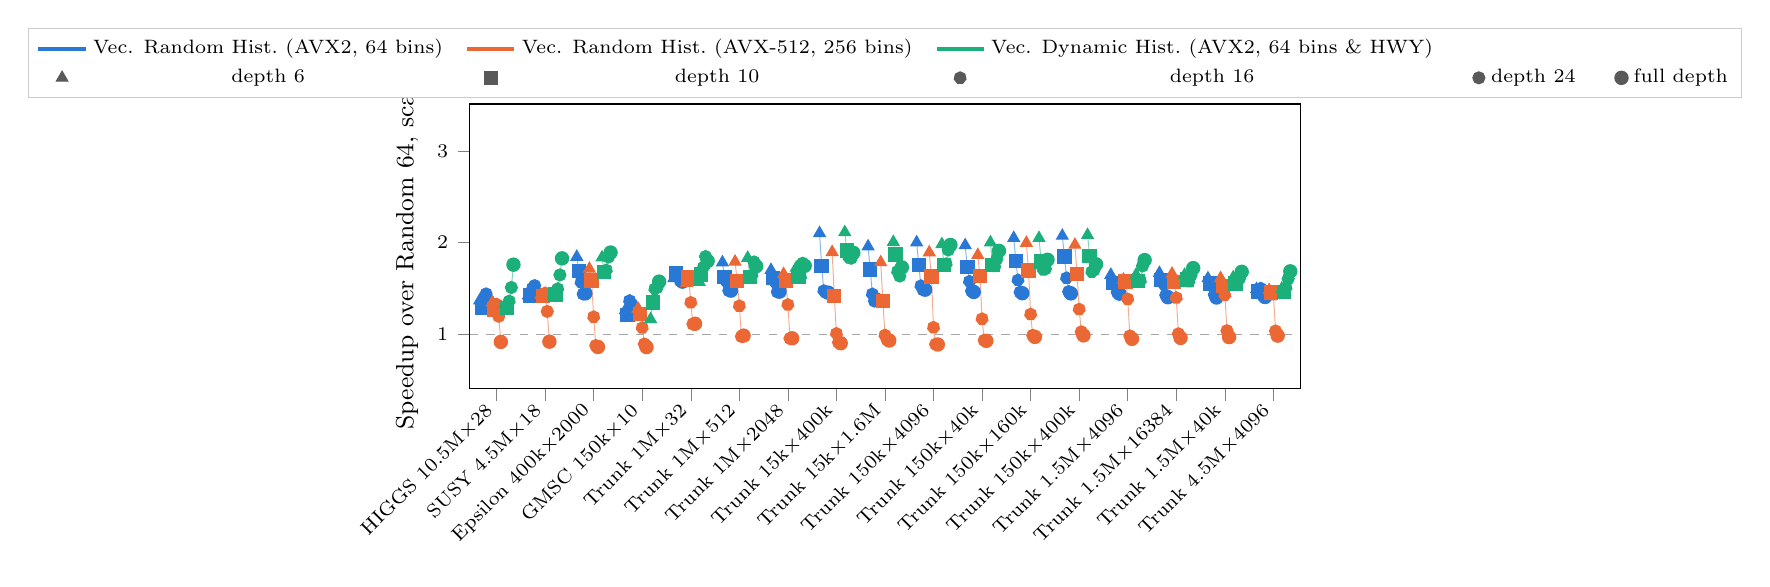
\begin{tikzpicture}
    \begin{axis}[
        width=\textwidth, height=5.2cm,
        xmin=0.45, xmax=17.55,
        ymin=0.41, ymax=3.51,
        xtick={1,2,3,4,5,6,7,8,9,10,11,12,13,14,15,16,17},
        xticklabels={HIGGS 10.5M$\times$28, SUSY 4.5M$\times$18, Epsilon 400k$\times$2000, GMSC 150k$\times$10, Trunk 1M$\times$32, Trunk 1M$\times$512, Trunk 1M$\times$2048, Trunk 15k$\times$400k, Trunk 15k$\times$1.6M, Trunk 150k$\times$4096, Trunk 150k$\times$40k, Trunk 150k$\times$160k, Trunk 150k$\times$400k, Trunk 1.5M$\times$4096, Trunk 1.5M$\times$16384, Trunk 1.5M$\times$40k, Trunk 4.5M$\times$4096},
        xticklabel style={rotate=45, anchor=east, font=\scriptsize},
        yticklabel style={font=\scriptsize},
        ylabel={Speedup over Random 64, scalar},
        ylabel style={font=\small},
        tick align=outside, tick pos=left,
        legend columns=5, legend style={font=\scriptsize, draw=gray!40,
            at={(0.5,1.02)}, anchor=south, /tikz/every even column/.append style={column sep=6pt}},
    ]
    \addplot[color=sp0, line width=0.35pt, opacity=0.55, mark=none, forget plot] coordinates {(0.652,1.3716) (0.696,1.2976) (0.740,1.3592) (0.784,1.4434) (0.828,1.3630)};
    \addplot[color=sp0, line width=0.35pt, opacity=0.55, mark=none, forget plot] coordinates {(1.652,1.4251) (1.696,1.4279) (1.740,1.5061) (1.784,1.5331) (1.828,1.4368)};
    \addplot[color=sp0, line width=0.35pt, opacity=0.55, mark=none, forget plot] coordinates {(2.652,1.8461) (2.696,1.6946) (2.740,1.5702) (2.784,1.4423) (2.828,1.4496)};
    \addplot[color=sp0, line width=0.35pt, opacity=0.55, mark=none, forget plot] coordinates {(3.652,1.2651) (3.696,1.2147) (3.740,1.3699) (3.784,1.3296) (3.828,1.2875)};
    \addplot[color=sp0, line width=0.35pt, opacity=0.55, mark=none, forget plot] coordinates {(4.652,1.6124) (4.696,1.6732) (4.740,1.6519) (4.784,1.5866) (4.828,1.5769)};
    \addplot[color=sp0, line width=0.35pt, opacity=0.55, mark=none, forget plot] coordinates {(5.652,1.7857) (5.696,1.6263) (5.740,1.5717) (5.784,1.4789) (5.828,1.4792)};
    \addplot[color=sp0, line width=0.35pt, opacity=0.55, mark=none, forget plot] coordinates {(6.652,1.7029) (6.696,1.6192) (6.740,1.5685) (6.784,1.4655) (6.828,1.4683)};
    \addplot[color=sp0, line width=0.35pt, opacity=0.55, mark=none, forget plot] coordinates {(7.652,2.1044) (7.696,1.7489) (7.740,1.4783) (7.784,1.4586) (7.828,1.4573)};
    \addplot[color=sp0, line width=0.35pt, opacity=0.55, mark=none, forget plot] coordinates {(8.652,1.9590) (8.696,1.7105) (8.740,1.4418) (8.784,1.3657) (8.828,1.3807)};
    \addplot[color=sp0, line width=0.35pt, opacity=0.55, mark=none, forget plot] coordinates {(9.652,2.0035) (9.696,1.7601) (9.740,1.5314) (9.784,1.4893) (9.828,1.4894)};
    \addplot[color=sp0, line width=0.35pt, opacity=0.55, mark=none, forget plot] coordinates {(10.652,1.9721) (10.696,1.7340) (10.740,1.5799) (10.784,1.4748) (10.828,1.4646)};
    \addplot[color=sp0, line width=0.35pt, opacity=0.55, mark=none, forget plot] coordinates {(11.652,2.0511) (11.696,1.8027) (11.740,1.5938) (11.784,1.4621) (11.828,1.4509)};
    \addplot[color=sp0, line width=0.35pt, opacity=0.55, mark=none, forget plot] coordinates {(12.652,2.0753) (12.696,1.8497) (12.740,1.6175) (12.784,1.4680) (12.828,1.4489)};
    \addplot[color=sp0, line width=0.35pt, opacity=0.55, mark=none, forget plot] coordinates {(13.652,1.6500) (13.696,1.5615) (13.740,1.5531) (13.784,1.4635) (13.828,1.4464)};
    \addplot[color=sp0, line width=0.35pt, opacity=0.55, mark=none, forget plot] coordinates {(14.652,1.6705) (14.696,1.5970) (14.740,1.5496) (14.784,1.4297) (14.828,1.4070)};
    \addplot[color=sp0, line width=0.35pt, opacity=0.55, mark=none, forget plot] coordinates {(15.652,1.6124) (15.696,1.5568) (15.740,1.5596) (15.784,1.4352) (15.828,1.4043)};
    \addplot[color=sp0, line width=0.35pt, opacity=0.55, mark=none, forget plot] coordinates {(16.652,1.4949) (16.696,1.4712) (16.740,1.5039) (16.784,1.4253) (16.828,1.4094)};
    \addplot[color=sp0, mark=triangle*, mark size=2.4pt, only marks, forget plot] coordinates {(0.652,1.3716) (1.652,1.4251) (2.652,1.8461) (3.652,1.2651) (4.652,1.6124) (5.652,1.7857) (6.652,1.7029) (7.652,2.1044) (8.652,1.9590) (9.652,2.0035) (10.652,1.9721) (11.652,2.0511) (12.652,2.0753) (13.652,1.6500) (14.652,1.6705) (15.652,1.6124) (16.652,1.4949)};
    \addplot[color=sp0, mark=square*, mark size=2.4pt, only marks, forget plot] coordinates {(0.696,1.2976) (1.696,1.4279) (2.696,1.6946) (3.696,1.2147) (4.696,1.6732) (5.696,1.6263) (6.696,1.6192) (7.696,1.7489) (8.696,1.7105) (9.696,1.7601) (10.696,1.7340) (11.696,1.8027) (12.696,1.8497) (13.696,1.5615) (14.696,1.5970) (15.696,1.5568) (16.696,1.4712)};
    \addplot[color=sp0, mark=heptagon*, mark size=2.4pt, only marks, forget plot] coordinates {(0.740,1.3592) (1.740,1.5061) (2.740,1.5702) (3.740,1.3699) (4.740,1.6519) (5.740,1.5717) (6.740,1.5685) (7.740,1.4783) (8.740,1.4418) (9.740,1.5314) (10.740,1.5799) (11.740,1.5938) (12.740,1.6175) (13.740,1.5531) (14.740,1.5496) (15.740,1.5596) (16.740,1.5039)};
    \addplot[color=sp0, mark=octagon*, mark size=2.4pt, only marks, forget plot] coordinates {(0.784,1.4434) (1.784,1.5331) (2.784,1.4423) (3.784,1.3296) (4.784,1.5866) (5.784,1.4789) (6.784,1.4655) (7.784,1.4586) (8.784,1.3657) (9.784,1.4893) (10.784,1.4748) (11.784,1.4621) (12.784,1.4680) (13.784,1.4635) (14.784,1.4297) (15.784,1.4352) (16.784,1.4253)};
    \addplot[color=sp0, mark=*, mark size=2.4pt, only marks, forget plot] coordinates {(0.828,1.3630) (1.828,1.4368) (2.828,1.4496) (3.828,1.2875) (4.828,1.5769) (5.828,1.4792) (6.828,1.4683) (7.828,1.4573) (8.828,1.3807) (9.828,1.4894) (10.828,1.4646) (11.828,1.4509) (12.828,1.4489) (13.828,1.4464) (14.828,1.4070) (15.828,1.4043) (16.828,1.4094)};
    \addplot[color=sp1, line width=0.35pt, opacity=0.55, mark=none, forget plot] coordinates {(0.912,1.3504) (0.956,1.2727) (1.000,1.3307) (1.044,1.1999) (1.088,0.9212)};
    \addplot[color=sp1, line width=0.35pt, opacity=0.55, mark=none, forget plot] coordinates {(1.912,1.4303) (1.956,1.4228) (2.000,1.4525) (2.044,1.2530) (2.088,0.9237)};
    \addplot[color=sp1, line width=0.35pt, opacity=0.55, mark=none, forget plot] coordinates {(2.912,1.7158) (2.956,1.5901) (3.000,1.1938) (3.044,0.8813) (3.088,0.8660)};
    \addplot[color=sp1, line width=0.35pt, opacity=0.55, mark=none, forget plot] coordinates {(3.912,1.2825) (3.956,1.2268) (4.000,1.0754) (4.044,0.8982) (4.088,0.8650)};
    \addplot[color=sp1, line width=0.35pt, opacity=0.55, mark=none, forget plot] coordinates {(4.912,1.5616) (4.956,1.6205) (5.000,1.3503) (5.044,1.1155) (5.088,1.1183)};
    \addplot[color=sp1, line width=0.35pt, opacity=0.55, mark=none, forget plot] coordinates {(5.912,1.7935) (5.956,1.5847) (6.000,1.3134) (6.044,0.9806) (6.088,0.9896)};
    \addplot[color=sp1, line width=0.35pt, opacity=0.55, mark=none, forget plot] coordinates {(6.912,1.6587) (6.956,1.5882) (7.000,1.3265) (7.044,0.9584) (7.088,0.9605)};
    \addplot[color=sp1, line width=0.35pt, opacity=0.55, mark=none, forget plot] coordinates {(7.912,1.8978) (7.956,1.4182) (8.000,1.0124) (8.044,0.9155) (8.088,0.9069)};
    \addplot[color=sp1, line width=0.35pt, opacity=0.55, mark=none, forget plot] coordinates {(8.912,1.7868) (8.956,1.3692) (9.000,0.9948) (9.044,0.9447) (9.088,0.9361)};
    \addplot[color=sp1, line width=0.35pt, opacity=0.55, mark=none, forget plot] coordinates {(9.912,1.8945) (9.956,1.6344) (10.000,1.0790) (10.044,0.8958) (10.088,0.8927)};
    \addplot[color=sp1, line width=0.35pt, opacity=0.55, mark=none, forget plot] coordinates {(10.912,1.8657) (10.956,1.6388) (11.000,1.1720) (11.044,0.9387) (11.088,0.9329)};
    \addplot[color=sp1, line width=0.35pt, opacity=0.55, mark=none, forget plot] coordinates {(11.912,1.9978) (11.956,1.6964) (12.000,1.2230) (12.044,0.9925) (12.088,0.9756)};
    \addplot[color=sp1, line width=0.35pt, opacity=0.55, mark=none, forget plot] coordinates {(12.912,1.9769) (12.956,1.6606) (13.000,1.2767) (13.044,1.0302) (13.088,0.9923)};
    \addplot[color=sp1, line width=0.35pt, opacity=0.55, mark=none, forget plot] coordinates {(13.912,1.5982) (13.956,1.5769) (14.000,1.3875) (14.044,0.9860) (14.088,0.9544)};
    \addplot[color=sp1, line width=0.35pt, opacity=0.55, mark=none, forget plot] coordinates {(14.912,1.6622) (14.956,1.5707) (15.000,1.4020) (15.044,1.0090) (15.088,0.9643)};
    \addplot[color=sp1, line width=0.35pt, opacity=0.55, mark=none, forget plot] coordinates {(15.912,1.6145) (15.956,1.5316) (16.000,1.4322) (16.044,1.0426) (16.088,0.9736)};
    \addplot[color=sp1, line width=0.35pt, opacity=0.55, mark=none, forget plot] coordinates {(16.912,1.4842) (16.956,1.4589) (17.000,1.4371) (17.044,1.0396) (17.088,0.9893)};
    \addplot[color=sp1, mark=triangle*, mark size=2.4pt, only marks, forget plot] coordinates {(0.912,1.3504) (1.912,1.4303) (2.912,1.7158) (3.912,1.2825) (4.912,1.5616) (5.912,1.7935) (6.912,1.6587) (7.912,1.8978) (8.912,1.7868) (9.912,1.8945) (10.912,1.8657) (11.912,1.9978) (12.912,1.9769) (13.912,1.5982) (14.912,1.6622) (15.912,1.6145) (16.912,1.4842)};
    \addplot[color=sp1, mark=square*, mark size=2.4pt, only marks, forget plot] coordinates {(0.956,1.2727) (1.956,1.4228) (2.956,1.5901) (3.956,1.2268) (4.956,1.6205) (5.956,1.5847) (6.956,1.5882) (7.956,1.4182) (8.956,1.3692) (9.956,1.6344) (10.956,1.6388) (11.956,1.6964) (12.956,1.6606) (13.956,1.5769) (14.956,1.5707) (15.956,1.5316) (16.956,1.4589)};
    \addplot[color=sp1, mark=heptagon*, mark size=2.4pt, only marks, forget plot] coordinates {(1.000,1.3307) (2.000,1.4525) (3.000,1.1938) (4.000,1.0754) (5.000,1.3503) (6.000,1.3134) (7.000,1.3265) (8.000,1.0124) (9.000,0.9948) (10.000,1.0790) (11.000,1.1720) (12.000,1.2230) (13.000,1.2767) (14.000,1.3875) (15.000,1.4020) (16.000,1.4322) (17.000,1.4371)};
    \addplot[color=sp1, mark=octagon*, mark size=2.4pt, only marks, forget plot] coordinates {(1.044,1.1999) (2.044,1.2530) (3.044,0.8813) (4.044,0.8982) (5.044,1.1155) (6.044,0.9806) (7.044,0.9584) (8.044,0.9155) (9.044,0.9447) (10.044,0.8958) (11.044,0.9387) (12.044,0.9925) (13.044,1.0302) (14.044,0.9860) (15.044,1.0090) (16.044,1.0426) (17.044,1.0396)};
    \addplot[color=sp1, mark=*, mark size=2.4pt, only marks, forget plot] coordinates {(1.088,0.9212) (2.088,0.9237) (3.088,0.8660) (4.088,0.8650) (5.088,1.1183) (6.088,0.9896) (7.088,0.9605) (8.088,0.9069) (9.088,0.9361) (10.088,0.8927) (11.088,0.9329) (12.088,0.9756) (13.088,0.9923) (14.088,0.9544) (15.088,0.9643) (16.088,0.9736) (17.088,0.9893)};
    \addplot[color=sp2, line width=0.35pt, opacity=0.55, mark=none, forget plot] coordinates {(1.172,1.3269) (1.216,1.2922) (1.260,1.3655) (1.304,1.5130) (1.348,1.7617)};
    \addplot[color=sp2, line width=0.35pt, opacity=0.55, mark=none, forget plot] coordinates {(2.172,1.4256) (2.216,1.4363) (2.260,1.4997) (2.304,1.6499) (2.348,1.8302)};
    \addplot[color=sp2, line width=0.35pt, opacity=0.55, mark=none, forget plot] coordinates {(3.172,1.8387) (3.216,1.6845) (3.260,1.7023) (3.304,1.8444) (3.348,1.8938)};
    \addplot[color=sp2, line width=0.35pt, opacity=0.55, mark=none, forget plot] coordinates {(4.172,1.1679) (4.216,1.3495) (4.260,1.4980) (4.304,1.5115) (4.348,1.5771)};
    \addplot[color=sp2, line width=0.35pt, opacity=0.55, mark=none, forget plot] coordinates {(5.172,1.5738) (5.216,1.6559) (5.260,1.7339) (5.304,1.8494) (5.348,1.8016)};
    \addplot[color=sp2, line width=0.35pt, opacity=0.55, mark=none, forget plot] coordinates {(6.172,1.8352) (6.216,1.6264) (6.260,1.6480) (6.304,1.7906) (6.348,1.7443)};
    \addplot[color=sp2, line width=0.35pt, opacity=0.55, mark=none, forget plot] coordinates {(7.172,1.7272) (7.216,1.6332) (7.260,1.6302) (7.304,1.7769) (7.348,1.7491)};
    \addplot[color=sp2, line width=0.35pt, opacity=0.55, mark=none, forget plot] coordinates {(8.172,2.1140) (8.216,1.9145) (8.260,1.8378) (8.304,1.8318) (8.348,1.8900)};
    \addplot[color=sp2, line width=0.35pt, opacity=0.55, mark=none, forget plot] coordinates {(9.172,2.0072) (9.216,1.8732) (9.260,1.6884) (9.304,1.6376) (9.348,1.7319)};
    \addplot[color=sp2, line width=0.35pt, opacity=0.55, mark=none, forget plot] coordinates {(10.172,1.9835) (10.216,1.7561) (10.260,1.7704) (10.304,1.9219) (10.348,1.9761)};
    \addplot[color=sp2, line width=0.35pt, opacity=0.55, mark=none, forget plot] coordinates {(11.172,2.0037) (11.216,1.7600) (11.260,1.7460) (11.304,1.8246) (11.348,1.9116)};
    \addplot[color=sp2, line width=0.35pt, opacity=0.55, mark=none, forget plot] coordinates {(12.172,2.0506) (12.216,1.7981) (12.260,1.7079) (12.304,1.7159) (12.348,1.8146)};
    \addplot[color=sp2, line width=0.35pt, opacity=0.55, mark=none, forget plot] coordinates {(13.172,2.0832) (13.216,1.8579) (13.260,1.6839) (13.304,1.7031) (13.348,1.7662)};
    \addplot[color=sp2, line width=0.35pt, opacity=0.55, mark=none, forget plot] coordinates {(14.172,1.6519) (14.216,1.5814) (14.260,1.5872) (14.304,1.7471) (14.348,1.8110)};
    \addplot[color=sp2, line width=0.35pt, opacity=0.55, mark=none, forget plot] coordinates {(15.172,1.6493) (15.216,1.6009) (15.260,1.5803) (15.304,1.6475) (15.348,1.7241)};
    \addplot[color=sp2, line width=0.35pt, opacity=0.55, mark=none, forget plot] coordinates {(16.172,1.6220) (16.216,1.5549) (16.260,1.5805) (16.304,1.6147) (16.348,1.6843)};
    \addplot[color=sp2, line width=0.35pt, opacity=0.55, mark=none, forget plot] coordinates {(17.172,1.4989) (17.216,1.4655) (17.260,1.5105) (17.304,1.6079) (17.348,1.6889)};
    \addplot[color=sp2, mark=triangle*, mark size=2.4pt, only marks, forget plot] coordinates {(1.172,1.3269) (2.172,1.4256) (3.172,1.8387) (4.172,1.1679) (5.172,1.5738) (6.172,1.8352) (7.172,1.7272) (8.172,2.1140) (9.172,2.0072) (10.172,1.9835) (11.172,2.0037) (12.172,2.0506) (13.172,2.0832) (14.172,1.6519) (15.172,1.6493) (16.172,1.6220) (17.172,1.4989)};
    \addplot[color=sp2, mark=square*, mark size=2.4pt, only marks, forget plot] coordinates {(1.216,1.2922) (2.216,1.4363) (3.216,1.6845) (4.216,1.3495) (5.216,1.6559) (6.216,1.6264) (7.216,1.6332) (8.216,1.9145) (9.216,1.8732) (10.216,1.7561) (11.216,1.7600) (12.216,1.7981) (13.216,1.8579) (14.216,1.5814) (15.216,1.6009) (16.216,1.5549) (17.216,1.4655)};
    \addplot[color=sp2, mark=heptagon*, mark size=2.4pt, only marks, forget plot] coordinates {(1.260,1.3655) (2.260,1.4997) (3.260,1.7023) (4.260,1.4980) (5.260,1.7339) (6.260,1.6480) (7.260,1.6302) (8.260,1.8378) (9.260,1.6884) (10.260,1.7704) (11.260,1.7460) (12.260,1.7079) (13.260,1.6839) (14.260,1.5872) (15.260,1.5803) (16.260,1.5805) (17.260,1.5105)};
    \addplot[color=sp2, mark=octagon*, mark size=2.4pt, only marks, forget plot] coordinates {(1.304,1.5130) (2.304,1.6499) (3.304,1.8444) (4.304,1.5115) (5.304,1.8494) (6.304,1.7906) (7.304,1.7769) (8.304,1.8318) (9.304,1.6376) (10.304,1.9219) (11.304,1.8246) (12.304,1.7159) (13.304,1.7031) (14.304,1.7471) (15.304,1.6475) (16.304,1.6147) (17.304,1.6079)};
    \addplot[color=sp2, mark=*, mark size=2.4pt, only marks, forget plot] coordinates {(1.348,1.7617) (2.348,1.8302) (3.348,1.8938) (4.348,1.5771) (5.348,1.8016) (6.348,1.7443) (7.348,1.7491) (8.348,1.8900) (9.348,1.7319) (10.348,1.9761) (11.348,1.9116) (12.348,1.8146) (13.348,1.7662) (14.348,1.8110) (15.348,1.7241) (16.348,1.6843) (17.348,1.6889)};
    \addplot[color=sp0, mark=none, line width=1.4pt] coordinates {(-9,1) (-8,1)};
    \addlegendentry{Vec. Random Hist.\ (AVX2, 64 bins)}
    \addplot[color=sp1, mark=none, line width=1.4pt] coordinates {(-9,1) (-8,1)};
    \addlegendentry{Vec. Random Hist.\ (AVX-512, 256 bins)}
    \addplot[color=sp2, mark=none, line width=1.4pt] coordinates {(-9,1) (-8,1)};
    \addlegendentry{Vec. Dynamic Hist.\ (AVX2, 64 bins \& HWY)}
    \addlegendimage{empty legend}
    \addlegendentry{}
    \addlegendimage{empty legend}
    \addlegendentry{}
    \addplot[color=black!65, mark=triangle*, mark size=2.4pt, only marks] coordinates {(-9,1)};
    \addlegendentry{depth 6}
    \addplot[color=black!65, mark=square*, mark size=2.4pt, only marks] coordinates {(-9,1)};
    \addlegendentry{depth 10}
    \addplot[color=black!65, mark=heptagon*, mark size=2.4pt, only marks] coordinates {(-9,1)};
    \addlegendentry{depth 16}
    \addplot[color=black!65, mark=octagon*, mark size=2.4pt, only marks] coordinates {(-9,1)};
    \addlegendentry{depth 24}
    \addplot[color=black!65, mark=*, mark size=2.4pt, only marks] coordinates {(-9,1)};
    \addlegendentry{full depth}
    \draw[gray!70, dashed, line width=0.6pt] (axis cs:0.45,1) -- (axis cs:17.55,1);
    \end{axis}
    \end{tikzpicture}
    \caption{Speedup over random histograms, 64 bins, scalar binner; layout as Figure~\ref{fig:speedup-by-depth-vs-exact}.}
    \label{fig:speedup-by-depth-vs-random64}
\end{figure*}
